%This work is licensed under Creative Commons Attribution-NonCommercial-ShareAlike 4.0 International. To view a copy of this license, visit https://creativecommons.org/licenses/by-nc-sa/4.0

\documentclass[12pt]{exam}
\newcommand{\semanticversion}{v1.0.0}               % Release version
\newcommand{\studentone}{Gage Linville}			    % Enter your name
\title{European Corn Borer Texas Quarantine Reference}			    % Title of the project
\newcommand{\creationdate}{May 24th, 2025}         % Creation date
%\newcommand{\revisiondate}{May 24th, 2025}           % Revision date
							
%-------------------------------------------------------------------------------------
%  PACKAGES
%-------------------------------------------------------------------------------------
\usepackage{graphicx}	
\usepackage{fourier} % Font file
\usepackage{titlesec} % Package that allows for a period to be placed after a section number

%-------------------------------------------------------------------------------------
%  GRAPHICS PATH
%-------------------------------------------------------------------------------------
\graphicspath{{figures/}}					      % Put your figures in a folder called figures

%-------------------------------------------------------------------------------------
% FUNCTIONS FOR IMPORTING FIGURES
%-------------------------------------------------------------------------------------
\newcommand{\placefigure}[1]{\centerline{\includegraphics[width=2 in]{#1}}} 
\newcommand{\placefigureandscale}[2]{\centerline{\includegraphics[width=#2 in]{#1}}} 

%-------------------------------------------------------------------------------------
% ADDITIONAL COMMANDS
%-------------------------------------------------------------------------------------
\renewcommand{\labelenumi}{\alph{enumi})}
\titlelabel{\thetitle.\quad} % Function for executing period after section number
%-------------------------------------------------------------------------------------
% TITLE PAGE MACRO
%-------------------------------------------------------------------------------------
\makeatletter
\def\maketitle{%
  \null
  \thispagestyle{empty}
  \begin{center}\leavevmode
       \normalfont
       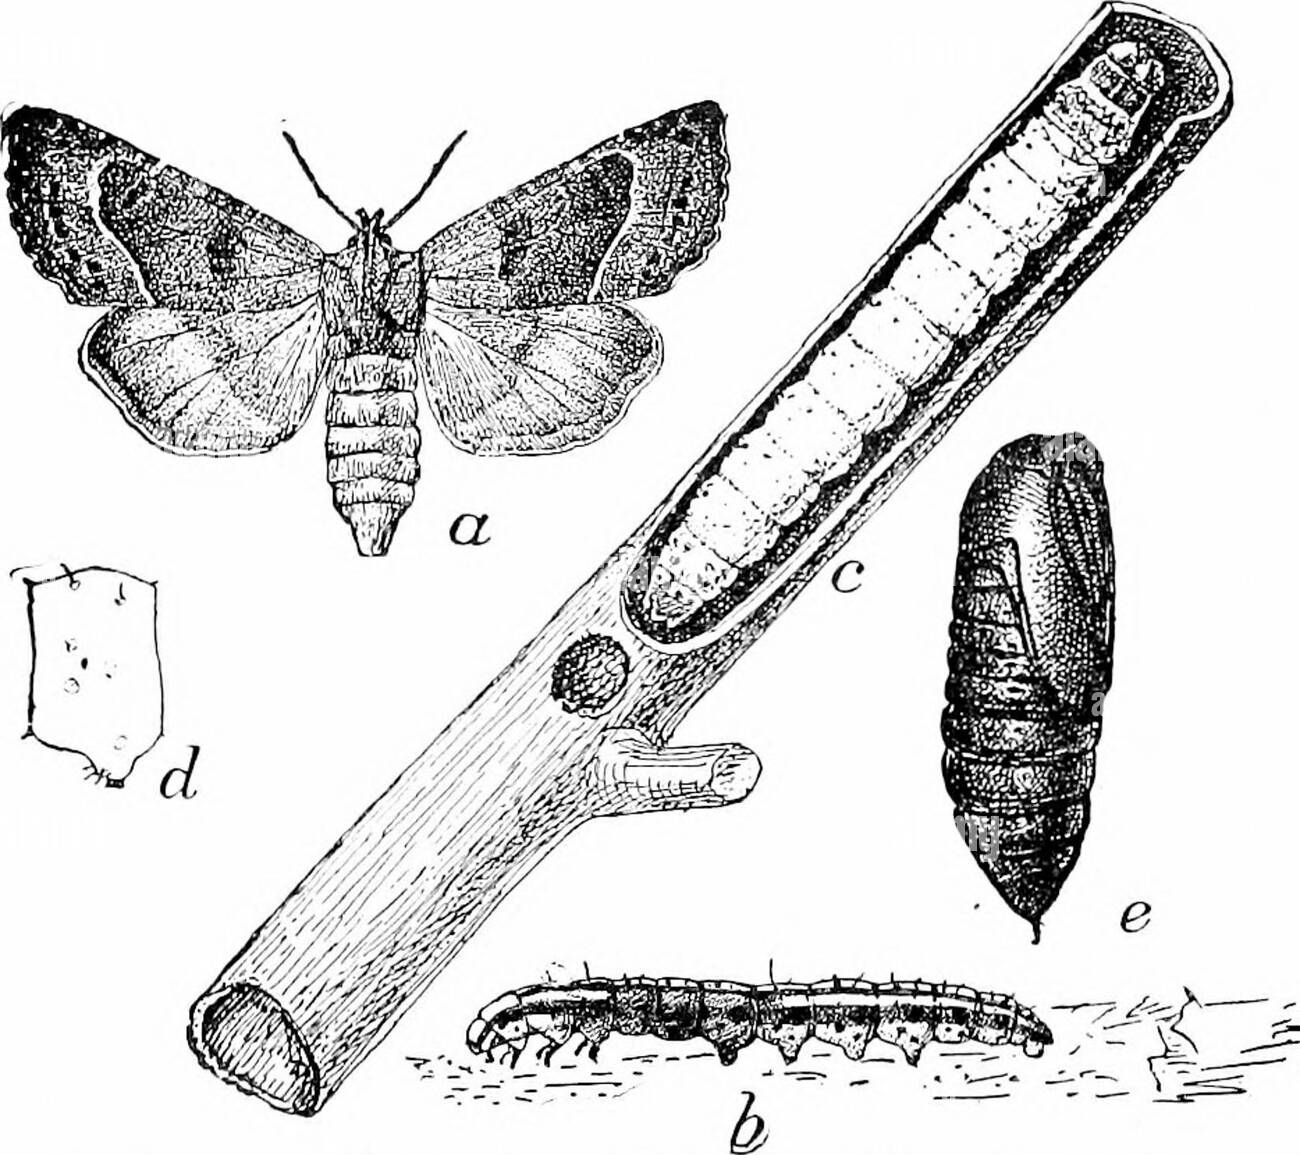
\includegraphics[width=0.40\columnwidth]{figures/Image.png}
	\rule{\linewidth}{0.2 mm} \\[0.4 cm]
	{ \huge \bfseries \@title}\\
	\rule{\linewidth}{0.2 mm} \\[0.4 cm]

	\begin{minipage}{0.5\textwidth}
		 \begin{center}\large
			Compiled by: \studentone\\
            Created: \creationdate\\
%            Revised: \revisiondate\\
            \semanticversion\\
            \
			\end{center}
			\end{minipage}
   \end{center}
   \vfill
   \null
   \cleardoublepage
  }
\makeatother

%-------------------------------------------------------------------------------------
% START OF DOCUMENT
%-------------------------------------------------------------------------------------

\begin{document}
%\large 
\maketitle
%\frontmatter
\let\cleardoublepage\clearpage
%\mainmatter
\sloppy

%-------------------------------------------------------------------------------------
% CONTENTS
%-------------------------------------------------------------------------------------
\section*{Quarantined Pest:}
The quarantined pest is the European Corn Borer, \textit{Ostrinia nubilalis}.

\section*{Quarantine Regulations:}
The Texas Department of Agriculture's European corn borer quarantine regulations are found in the Texas Admin Code: Title 4, Chapter 19, Subchapter K, Rule §§19.110-19.113.

\section*{Quarantined Articles:}
\begin{enumerate}
\item The quarantined pest.
\item Corn, broomcorn, sorghums, and sudan grass plants and plant parts (including, but not limited to, seed and shelled grain, and stalks, ears, cobs, and all other parts, fragments, or debris).
\item Beans in the pod, beets, celery, pepper fruits, endive, swiss chard, and rhubarb (cut or plants with roots).
\item Cut flowers and entire plants of aster, chrysanthemum, dendranthema, pelargonium, calendula, cosmos, hollyhock, marigold, zinnia, Japanese hop, dahlia, and gladiolus.
\item Plants and plant parts of Cannabis spp.
\end{enumerate}

\section*{Geographic Areas Subject to Quarantine:}

\section{Outside Texas:}

\begin{enumerate}
\item  Alabama, Arkansas, Colorado, Connecticut, Delaware, Georgia, Illinois, Iowa, Indiana, Kansas, Kentucky, Louisiana, Maine, Maryland, Massachusetts, Michigan, Minnesota, Mississippi, Missouri, Montana, Nebraska, New Hampshire, New Jersey, New York, North Carolina, North Dakota, Ohio, Oklahoma, Pennsylvania, Rhode Island, South Carolina, South Dakota, Tennessee, Vermont, Virginia, West Virginia, Wisconsin, Wyoming.
\item The following counties in the State of Florida: Calhoun, Escambia, Gadsden, Hamilton, Holmes, Jackson, Jefferson, Madison, Okaloosa, and Santa Rosa.
\end{enumerate}

\section{Within Texas:}
\begin{enumerate}
\item Bailey, Carson, Castro, Dallam, Deaf Smith, Floyd, Gray, Hale, Hansford, Hartley, Hutchinson, Lamb, Lipscomb, Moore, Ochiltree, Oldham, Parmer, Potter, Randall, Roberts, Sherman, and Swisher County.
\end{enumerate}
\newpage
\textbf{References:}\\
1. TDA Website: https://texasagriculture.gov/Regulatory-Programs/Plant-Quality/Pest-and-Disease-Alerts/European-Corn-Borer
% Texas Admin Code Direct Link: https://texas-sos.appianportalsgov.com/rules-and-meetings?chapter=19&interface=VIEW_TAC&part=1&subchapter=K&title=4

\end{document}